\subsection{Logistic Regression}

Logistic Regression biner memodelkan probabilitas bersyarat kelas positif
$y = 1$ (pemesanan dibatalkan) terhadap fitur masukan $x \in \mathbb{R}^d$
melalui kombinasi linear (\textit{log-odds}) $z = b_0 + \sum_{j=1}^d b_j x_j = b^\top \tilde{x}$
dengan $\tilde{x} = [1, x^\top]^\top$ dan fungsi aktivasi sigmoid (Khodra, 2021):
\[
  P(y = 1 \mid x) = \sigma(z) = \frac{1}{1 + e^{-z}}.
\]
Pelatihan parameter $b$ dilakukan berdasarkan prinsip \textit{Maximum Likelihood
Estimation} (MLE) dengan memaksimumkan \textit{Log Joint Conditional Likelihood}
(LCL), yang ekuivalen dengan meminimalkan rata-rata \textit{negative log-loss}
ditambah suku regularisasi $R(b_{1:d})$ (Khodra, 2021):
\[
  \mathcal{L}(b) = -\frac{1}{n}\sum_{i=1}^{n} \Big[y_i \log p_i + (1 - y_i)\log(1 - p_i)\Big] + R(b_{1:d}),
\]
dengan $p_i = \sigma(b^\top \tilde{x}_i)$. Suku penalti hanya dikenakan pada bobot
fitur $w = b_{1:d}$ (tidak pada \textit{bias} $b_0$) untuk tiga varian:
\[
  R_{\text{L1}}(w) = \lambda \sum_{j=1}^{d} |w_j|, \qquad
  R_{\text{L2}}(w) = \frac{\lambda}{2} \sum_{j=1}^{d} w_j^2, \qquad
  R_{\text{EN}}(w) = \lambda \left( r \sum_{j=1}^{d} |w_j| + \frac{1 - r}{2} \sum_{j=1}^{d} w_j^2 \right),
\]
dengan $\lambda$ adalah \texttt{reg\_lambda} dan $r \in [0, 1]$ adalah
\texttt{l1\_ratio}.

\subsubsection{Implementasi}

Implementasi \textit{from scratch} berada pada berkas
\texttt{src/models/logistic\_regression.py} (337 baris) dan diintegrasikan
dengan antarmuka tim melalui kelas \texttt{LogisticRegression(BaseModel)},
konfigurasi \texttt{DEFAULT\_LOGREG\_CONFIGS}, serta
\texttt{get\_logreg\_preprocessing\_config()}. Pipeline \textit{preprocessing}
mengaktifkan standarisasi numerik, SMOTE pada himpunan latih, seleksi fitur, dan
PCA agar skala fitur seragam dan gradien tetap stabil.

Komponen utama di dalam kelas \texttt{LogisticRegression} meliputi:
\begin{itemize}
  \item \texttt{\_sigmoid}, \texttt{\_add\_intercept}, \texttt{log\_odds},
        \texttt{\_compute\_lcl}, \texttt{\_compute\_penalty}, dan
        \texttt{\_regularization\_grad}: melakukan pemotongan numerik
        (\textit{clipping}) pada logit $[-500, 500]$ dan probabilitas
        $[10^{-15}, 1 - 10^{-15}]$ untuk mencegah \textit{overflow}/\texttt{log(0)},
        serta menghitung nilai dan turunan penalti L1, L2, dan Elastic Net.
  \item \texttt{\_fit\_sga} dan \texttt{\_fit\_adam}: menyediakan dua metode
        optimasi, yakni \textit{Stochastic Gradient Ascent} (SGA) sesuai materi
        kuliah (Khodra, 2021) dan \textit{mini-batch Adam} sebagai metode
        optimasi tambahan (Kingma dan Ba, 2015). Keduanya mencatat riwayat
        \texttt{lcl\_history\_} serta \texttt{loss\_history\_} pada tiap
        \textit{epoch} melalui \texttt{\_record\_epoch} dan berhenti otomatis
        apabila perubahan \textit{loss} lebih kecil dari \texttt{tol}.
  \item \texttt{fit}, \texttt{predict\_proba}, \texttt{predict}, serta
        \texttt{save}/\texttt{load}: memetakan label target ke $\{0, 1\}$,
        memprediksi kelas dengan ambang \texttt{threshold} (bawaan $0{,}5$), dan
        mendukung serialisasi berbasis \texttt{joblib} (dengan cadangan
        \texttt{pickle}).
\end{itemize}

Pada SGA, pembaruan dilakukan secara sekuensial per sampel ($\tilde{x}_i$),
sehingga lintasan gradien cenderung berosilasi dan membutuhkan iterasi baris
dalam Python. Sebaliknya, \textbf{Adam} (\textit{Adaptive Moment Estimation})
mengoptimasi proses pelatihan lewat empat mekanisme (Kingma dan Ba, 2015):
(1) menghitung gradien secara vektorisasi per \textit{mini-batch} berukuran 256;
(2) mempertahankan momentum orde pertama $m_t = \beta_1 m_{t-1} + (1 - \beta_1) g_t$
($\beta_1 = 0{,}9$) agar arah pembaruan lebih halus; (3) mempertahankan estimasi
variansi gradien orde kedua $v_t = \beta_2 v_{t-1} + (1 - \beta_2) g_t^2$
($\beta_2 = 0{,}999$) untuk menyesuaikan ukuran langkah adaptif tiap parameter; dan
(4) menerapkan koreksi bias $\hat{m}_t, \hat{v}_t$ sehingga konvergensi awal
lebih stabil tanpa menuntut penyetelan \textit{learning rate} yang ketat.

\begin{lstlisting}
def _regularization_grad(self):
    w = self.b_[1:]
    if self.penalty == "l1":
        return self.reg_lambda * np.sign(w)
    if self.penalty == "l2":
        return self.reg_lambda * w
    if self.penalty == "elasticnet":
        return self.reg_lambda * (self.l1_ratio * np.sign(w) + (1.0 - self.l1_ratio) * w)
    return np.zeros_like(w)

def _fit_sga(self, X_bias, y_bin):
    rng = np.random.default_rng(self.random_state)
    use_reg = self.penalty not in (None, "none") and self.reg_lambda > 0.0
    for epoch in range(1, self.max_iter + 1):
        for idx in (rng.permutation(len(X_bias)) if self.shuffle else range(len(X_bias))):
            x_i = X_bias[idx]
            p_i = self._sigmoid(np.dot(self.b_, x_i))
            self.b_ += self.learning_rate * (y_bin[idx] - p_i) * x_i
            if use_reg:
                self.b_[1:] -= self.learning_rate * self._regularization_grad()
        if self._record_epoch(epoch, X_bias, y_bin):
            break

def _fit_adam(self, X_bias, y_bin):
    m, v = np.zeros(X_bias.shape[1]), np.zeros(X_bias.shape[1])
    t_step = 0
    for epoch in range(1, self.max_iter + 1):
        ...
        t_step += 1
        m = self.beta1 * m + (1.0 - self.beta1) * grad
        v = self.beta2 * v + (1.0 - self.beta2) * (grad ** 2)
        m_hat = m / (1.0 - self.beta1 ** t_step)
        v_hat = v / (1.0 - self.beta2 ** t_step)
        self.b_ -= self.learning_rate * m_hat / (np.sqrt(v_hat) + self.eps)
\end{lstlisting}

\subsubsection{Hasil dan Perbandingan dengan scikit-learn}

Eksperimen lengkap dijalankan melalui
\texttt{notebooks/logistic\_regression\_experiment.ipynb} menggunakan pembagian
data validasi 15\% (\texttt{random\_state=824}). Evaluasi 5-\textit{fold
Stratified Cross-Validation} pada himpunan latih (mencakup seluruh kombinasi
regularisasi dan \textit{optimizer} pada \texttt{DEFAULT\_LOGREG\_CONFIGS})
dirangkum pada Tabel~\ref{tab:logreg-cv}.

\begin{table}[htbp]
  \centering
  \caption{Hasil 5-\textit{Fold Stratified Cross-Validation} Logistic Regression \textit{from scratch}.}
  \label{tab:logreg-cv}
  \footnotesize
  \begin{tabular}{llccc}
    \toprule
    \textbf{Optimizer} & \textbf{Regularisasi} & \textbf{Epoch / LR} & \textbf{Mean Akurasi} & \textbf{Mean Macro-F1} \\
    \midrule
    SGA  & Tanpa penalti (\texttt{None}) & 20 / 0,01 & 0,75147 & 0,75121 $\pm$ 0,00402 \\
    SGA  & L1 ($\lambda = 10^{-4}$) & 20 / 0,01 & 0,75083 & 0,75056 $\pm$ 0,00445 \\
    SGA  & L2 ($\lambda = 10^{-4}$) & 20 / 0,01 & 0,74999 & 0,74971 $\pm$ 0,00433 \\
    SGA  & Elastic Net ($\lambda = 10^{-4}, r = 0{,}5$) & 20 / 0,01 & 0,74977 & 0,74948 $\pm$ 0,00388 \\
    Adam & L2 ($\lambda = 10^{-4}$, \texttt{bs}=256) & 30 / 0,02 & 0,75064 & 0,75051 $\pm$ 0,00496 \\
    Adam & Elastic Net ($\lambda = 10^{-4}, r = 0{,}5$) & 30 / 0,02 & 0,75093 & 0,75079 $\pm$ 0,00502 \\
    \bottomrule
  \end{tabular}
\end{table}

Selisih antar-konfigurasi pada validasi silang sangat tipis ($< 0{,}002$ pada
\textit{macro-F1}) karena fitur masukan sudah melalui \texttt{SelectKBest} dan
PCA sehingga dimensi fitur lebih kompak dan ortogonal. Konfigurasi terbaik dari
CV (\texttt{SGA}, \texttt{penalty=None}, \texttt{lr=0,01}, 20 \textit{epoch})
kemudian dilatih ulang hanya pada baris latih asli (\texttt{fit\_orig\_only=True})
dan diuji pada 4.081 baris validasi asli (2.741 kelas 0 dan 1.340 kelas 1)
melawan \texttt{sklearn.linear\_model.LogisticRegression(max\_iter=1000)}.
Hasil perbandingan disajikan pada Tabel~\ref{tab:logreg-sklearn} dan
Gambar~\ref{fig:logreg-eval}.

\begin{table}[htbp]
  \centering
  \caption{Perbandingan Logistic Regression \textit{from scratch} dan \texttt{scikit-learn} pada 4.081 sampel validasi asli.}
  \label{tab:logreg-sklearn}
  \footnotesize
  \begin{tabular}{lcccc}
    \toprule
    \textbf{Model} & \textbf{Akurasi} & \textbf{Presisi} & \textbf{Recall} & \textbf{Macro-F1} \\
    \midrule
    \texttt{LogisticRegression} (Scratch - SGA) & 0,77922 & 0,73833 & 0,50746 & 0,72441 \\
    \texttt{LogisticRegression} (Scikit-Learn)  & 0,78069 & 0,73446 & 0,52015 & 0,72830 \\
    \bottomrule
  \end{tabular}
\end{table}

\begin{figure}[htbp]
  \centering
  \begin{minipage}{0.46\textwidth}
    \centering
    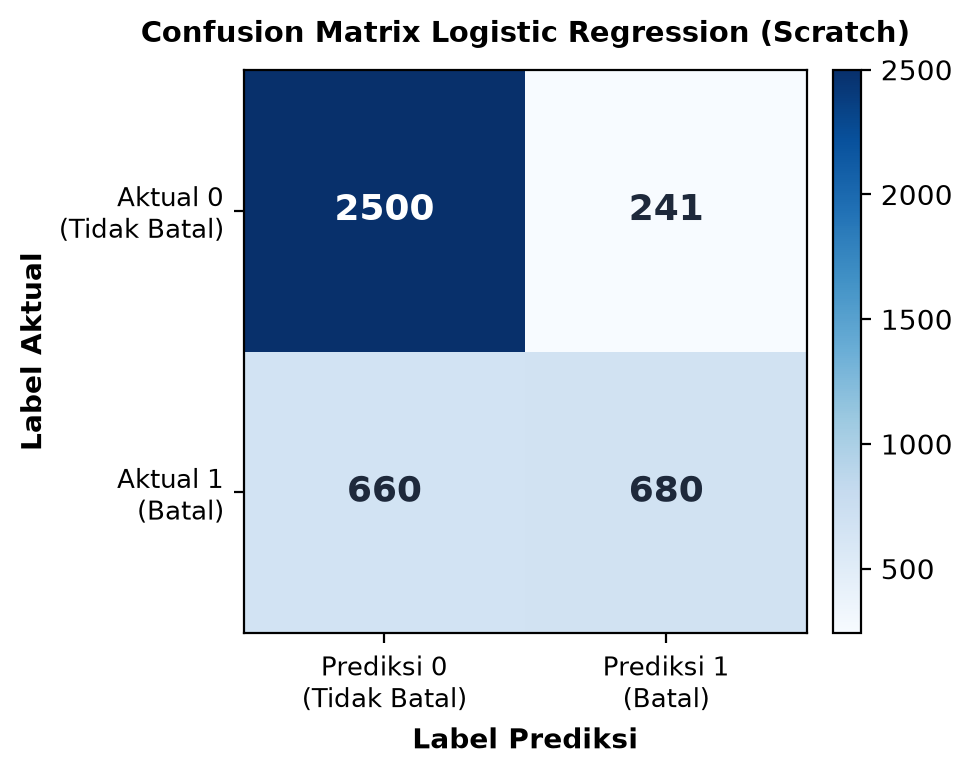
\includegraphics[width=\linewidth]{assets/logreg/logreg-cm.png}\\
    (a) \textit{Confusion matrix} model terbaik
  \end{minipage}\hfill
  \begin{minipage}{0.51\textwidth}
    \centering
    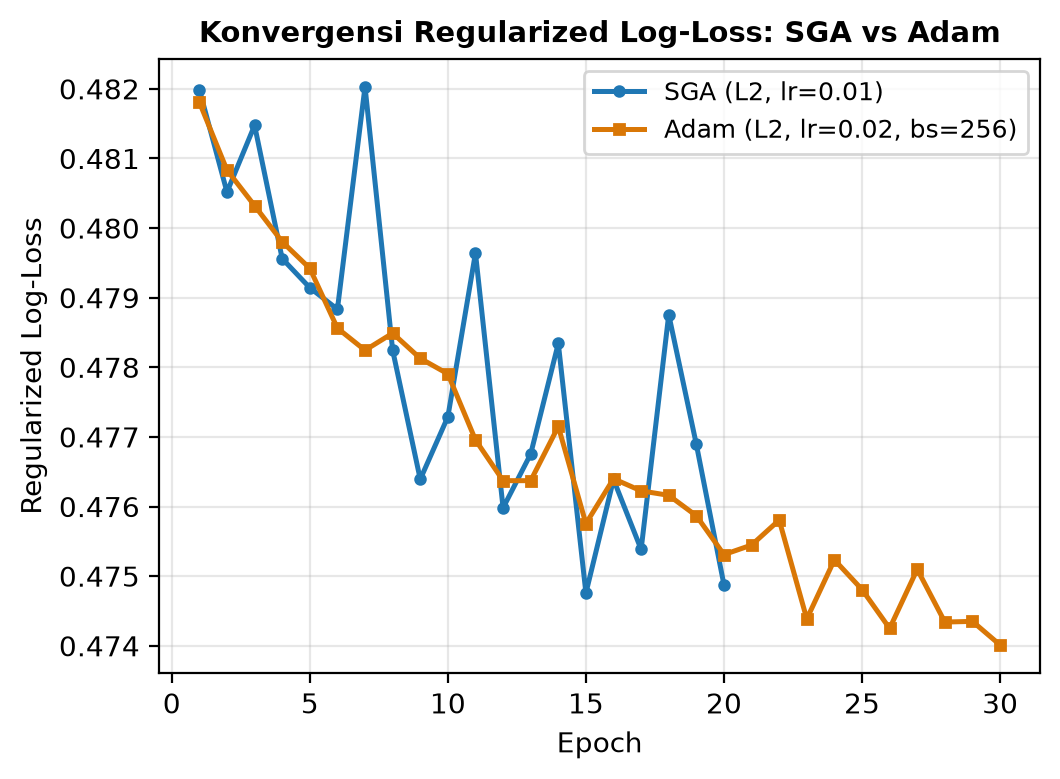
\includegraphics[width=\linewidth]{assets/logreg/logreg-loss.png}\\
    (b) Kurva konvergensi \textit{log-loss} SGA vs Adam
  \end{minipage}
  \caption{Evaluasi \textit{confusion matrix} pada himpunan validasi asli dan perbandingan konvergensi SGA terhadap mini-batch Adam.}
  \label{fig:logreg-eval}
\end{figure}

Secara kuantitatif, implementasi \textit{from scratch} sangat mendekati
pustaka referensi: selisih akurasi hanya 0,00147, \textit{macro-F1} berselisih
0,00389, tingkat kesepakatan prediksi (\textit{prediction agreement}) mencapai
\textbf{97,35\%}, dan \textit{cosine similarity} antara vektor bobot fitur kedua
model mencapai \textbf{0,99743}. Perbedaan kecil tersebut wajar karena
\texttt{scikit-learn} menggunakan \textit{solver} kuasi-Newton \texttt{lbfgs}
dengan regularisasi L2 bawaan hingga konvergen penuh, sedangkan model
\textit{from scratch} berhenti pada 20 \textit{epoch} SGA.

Dari Gambar~\ref{fig:logreg-eval}(a), diperoleh $\text{TN} = 2.500$,
$\text{FP} = 241$, $\text{FN} = 660$, dan $\text{TP} = 680$. Model mengenali
kelas mayoritas (tidak batal) dengan sangat baik (\textit{recall} $0{,}91$,
F1 $0{,}85$), tetapi lebih konservatif pada kelas positif (\textit{recall}
$0{,}51$, F1 $0{,}60$) karena distribusi kelas tidak seimbang dan pemisahan
antar-kelas di ruang fitur PCA bersifat non-linear. Sementara itu, perbandingan
SGA vs Adam berpenalti L2 ($\lambda = 10^{-4}$) pada Gambar~\ref{fig:logreg-eval}(b)
menunjukkan bahwa mini-batch Adam (30 \textit{epoch}) jauh lebih cepat secara
komputasi (\textbf{0,064 detik} dibanding \textbf{1,602 detik} pada SGA
20 \textit{epoch}, atau $\sim 25\times$ lebih cepat berkat vektorisasi batch) dan
mencapai \textit{regularized log-loss} latih lebih rendah (\textbf{0,47401} vs
\textbf{0,47487}), dengan akurasi validasi yang tetap sebanding (0,77162 vs
0,77824).

Terakhir, verifikasi penyimpanan model ke \texttt{output/logreg.pkl}
(berukuran \textbf{1,13 KB}) mengonfirmasi bobot hasil \textit{load} identik
dengan model sebelum disimpan. Inferensi pada seluruh 6.844 baris data uji di
\texttt{output/submission\_logreg.csv} menghasilkan distribusi prediksi
5.268 kelas 0 (76,97\%) dan 1.576 kelas 1 (23,03\%) yang konsisten dengan sifat
konservatif model terhadap kelas positif.
